%Top}ics for introduction / related work:
%1. One of the challenges faced by scientists is the data analysis and visualization of the large amounts of data generated by simulation codes on HPC resources.
%2. In situ processing offers a potential solution by circumventing the need to store all the raw data. 
%3. Most in situ analysis tasks operate infrequently or are triggered. Computing Lagrangian flow maps is unlike other analysis tasks and requires computation every cycles of the simulation - this places an overhead on the simulation code and raises questions of viability. 
%4. Lagrangian analysis has been extensively studied for ocean modeling in an offline setting and now efforts to support online analysis are being made.
%5. Reduced Lagrangian flow maps have been shown to be superior to traditional Eulerian subsampling for primarily analytical data sets, in theoretical settings or 2D flows, and compared using a single average error across all post hoc interpolated particles. 
%6. We believe reduced Lagrangian flow maps need to be explored for more real world time-varying vector fields to better understand their applicability, and more closely evalauted - both quantitatively and qualitatively - to understand efficacy characteristics.
%7. We strongly believe Lagrangian flow maps need to be evaluated in representative settings - integrated with a simulation code and executing on a supercomputer - to provide insight into viability.
%8. Given reduced Lagrangian flow maps are a new paradigm - it opens research opportunities along multiple axes - namely, sampling strategy, post hoc interpolation, ease of use (integration), performance (viability) and applicability (configuration settings, vector field type, etc). 
%9. Several works have advanced research along these axes - but none have considered viability in relation to simulation execution times or application to seismology or cosmology vector fields. Demonstration in this form we believe encourages wider adoption of the paradigm beyond the theoretical level.
%
%
%
%
High-performance computing resources play a key role in advancing computational science by enabling modeling of scientific phenomena at high spatiotemporal resolutions.
%
%Although HPC enables modeling of scientific phenomena at high spatiotemporal resolutions, the total data generated is prohibitively large.
%
A challenge with regard to studying the output of a simulation is the prohibitively large size of the total data generated.
%
Compromise in the form of storing a subset of the data can impact the extent and accuracy of subsequent post hoc exploratory analysis and visualization.
%
In particular, for accurate time-varying vector field analysis and visualization, access to the full spatiotemporal resolution is required.
%
Since storing the entire simulation output is expensive, scientists resort to temporal subsampling or lossy compression, and often limit analysis to individual time slices.
%
An emerging paradigm to address large data challenges is the use of in situ processing to perform runtime analysis/visualization or data reduction to support exploratory post hoc analysis.
%
%

%In situ Lagrangian analysis is an emerging paradigm to enable post hoc exploration of time-varying vector fields.
% and has presented research opportunities along multiple orthogonal axes.
%
Lagrangian analysis is a powerful tool to study time-varying vector fields and is widely employed for ocean modeling applications~\cite{VANSEBILLE201849}.
%
The notion of calculating a Lagrangian representation or \textit{flow map}, i.e., sets of particle trajectories, ``online'' (in situ) for ``offline'' (post hoc) exploration was first proposed by Vries et al.~\cite{vries2001calculating} for an ocean modeling simulation.
%
Figure~\ref{fig:sample} illustrates the approach.
%
The black trajectories are first extracted in situ and are referred to as \textit{basis} trajectories.
%
They are used to reconstruct the red trajectory post hoc.
%
The end location of the red trajectory deviates by a margin of error from the ground truth and is the result of using a Lagrangian-based advection scheme \textit{L}, i.e., a technique to interpolate flow maps.
%
The quality of reconstruction depends on the vector field as well as configuration specifics such as sampling strategy and frequency of storage. 
%
More recently, multiple works have advanced Lagrangian research along axes such as strategies for in situ extraction of reduced Lagrangian representations~\cite{agranovsky2014improved}\cite{rapp2019void}\cite{sane2020scalable}, post hoc reconstruction~\cite{chandler2015interpolation}\cite{sane2019interpolation}\cite{Jakob20}, and theoretical error analysis~\cite{bujack2015lagrangian}\cite{chandler2016analysis}\cite{hummel2016error}.
%Agranovsky et al.~\cite{agranovsky2014improved} proposed computing reduced Lagrangian representations using in situ processing to access the complete spatiotemporal resolution of the simulation.
%
%More recently, Pascal et al.~\cite{envirvis.20171099,siegfried2019tropical} used embedded routines to compute reduced Lagrangian data in order to explore coastal upwelling activity and visualize a derived scalar field representing trajectory density.
%
Existing evaluations of reduced Lagrangian representations, although often conducted in theoretical in situ environments using analytical data sets where ground truths are known, have been encouraging and show that performance characteristics vary from case to case. 
%
%Existing evaluations, although on a limited set of applications and primarily conducted in theoretical in situ settings, are promising.
%
Thus, the application of reduced Lagrangian representations to a broader range of real-world simulation vector fields, and in practice, is of keen interest to us.
%
%However, existing evaluations of reduced Lagrangian representations are on a limited, and often analytical, set of applications, most set in theoretical in situ settings. %~\cite{agranovsky2014improved}\cite{sane2018revisiting}.
%
%However, in addition to only preliminary evaluations of efficacy on a limited, and often analytical, set of data, these studies are performed in theoretical settings.
%
%Thus, the use of reduced Lagrangian representations for a broader range of applications and in practice, remains not well understood.
%
%In this paper, we investigate Lagrangian representations for time-varying vector fields produced by cosmology and seismology simulations in representative HPC settings.
%

In this paper, our contribution is an investigation of reduced Lagrangian representations to encode the self-gravitating gas dynamics of a cosmology simulation and seismic wave propagation in a seisomology simulation.
%
For the self-gravitating gas dynamics vector field, our experiments show that Lagrangian representations can enable accurate analysis of particle evolution and structure formation in the simulation.
%
Further, we show that reconstruction accuracy statistically improves as temporal sparsity increases, providing an opportunity for increased data reduction.
%
For the seismic wave propagation vector field, we find that Lagrangian representations are well suited to capture transient wave patterns in the flow, resulting in accurate reconstructions for several data reduction options.
%
Overall, our experiments show that Lagrangian representations offer high data reductions of the time-varying vector fields considered for a small loss of accuracy, are viable to compute in situ, and should be considered more widely for time-varying vector field analysis.  
%accurate reconstruction of the time evolutions of the simulation  
%
%
%choices for both spatial and temporal sampling can impact the reconstruction
%
%
%We study the efficacy of Lagrangian representations by conducting a statistical evaluation across a range of spatiotemporal configurations as well as a qualitative evaluation for varying data reduction factors. %for cosmology and seismology applications.
%
%Our experiments evaluate viability by measuring in situ encumbrance in representative settings, i.e., a tightly-coupled integration with the simulation code and execution on HPC resources.
%
%Our results show that Lagrangian representations offer strong data storage-accuracy propositions for time-varying analysis of the vector fields studied and require a low cost to extract. %using HPC resources.
%
%Our experiments evaluate the cost of a tightly-coupled in situ processing integration with each simulation code using Ascent and execution on HPC resources.
%\item An evaluation of in situ encumbrance in representative settings, i.e., tightly-coupled integration with a simulation and use of HPC resources at scale.
%\item A benchmarking study to measure in situ encumbrance using Cloverleaf3D.
%\end{tightItemize}

\begin{figure}[!t]
\centering
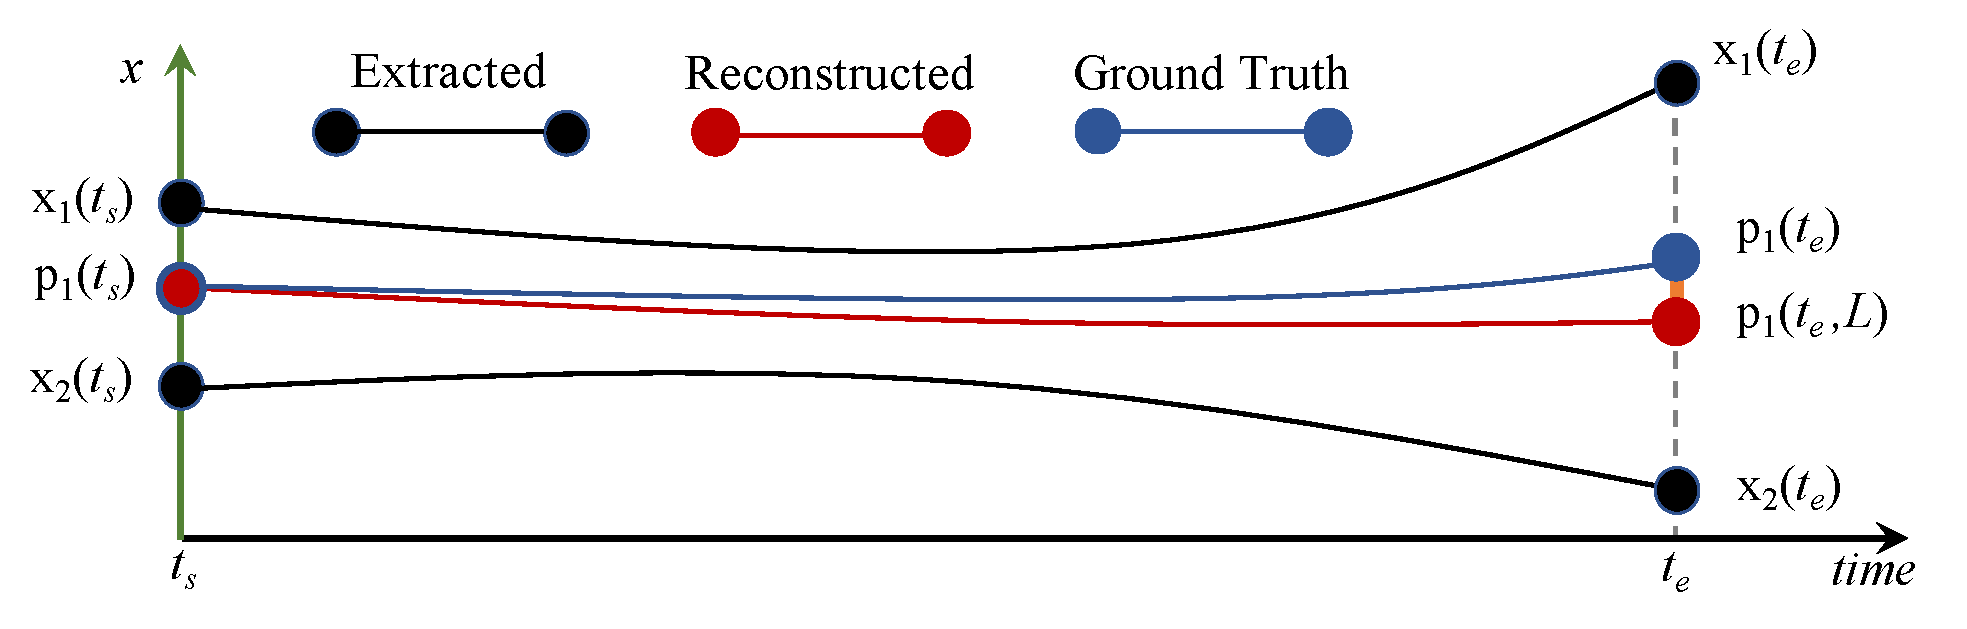
\includegraphics[width=0.9\linewidth]{Images/sample.pdf}
\vspace{-5mm}
\caption{Notional space-time visualization of Lagrangian representations for a time-varying 1D flow. The black trajectories are computed in situ and encode the behavior of the vector field between start time \textit{t$_{s}$} and end time \textit{t$_{e}$}. In a post hoc setting, a Lagrangian-based advection scheme \textit{L} is used to interpolate the extracted data and calculate the trajectory of a new particle p$_{1}$ . The red trajectory is the reconstructed trajectory and the blue trajectory is the ground truth.}
\vspace{-5mm}
\label{fig:sample}
\end{figure}

%First, we explore the use of Lagrangian representations to encode particle transport behavior of baryonic matter evolving under self-gravitating gas dynamics in the Nyx cosmology simulation~\cite{almgren2013nyx}.
%
%Next, we evaluate the potential of Lagrangian representations to encode the behavior of a fourth-order seismic wave propagation simulation SW4~\cite{petersson2015wave}. 
%
%In addition to investigating the use of Lagrangian representations for these vector fields, our study improves on prior efficacy and performance evaluations.
%
%We present the first statistical analysis of reconstruction accuracy for a range of spatiotemporal configurations as well as the first qualitative comparison to the traditional Eulerian approach. 
%
%Finally, we measure performance in a representative setting by considering integrated in situ infrastructure and execution using both GPUs and CPUs on a supercomputer.

%toring the time-varying vector field using a reduced Lagrangian representation is 
%
%In this paper, we focus on the axes of viability and efficacy. 
%
%Prior studies of reduced Lagrangian flow maps have shown improved accuracy-storage propositions compared to the traditional Eulerian paradigm under sparse temporal settings.
%
%However, only theoretical in situ settings, i.e., data sets are loaded from disk, on a single compute node or at small scale have been considered.
%
%With respect to type of time-varying vector field, either analytical data sets or data from climate and ocean modeling simulations has been considered.
%
%Further, for evaluation of reconstruction accuracy, comparisons to the Eulerian paradigm have been limited to quantitative analysis using a single average error.
%

%To determine viability, it is essential to evaluate the cost of in situ Lagrangian analysis in relation to the simulation execution time. 
%%
%In situ computation of a Lagrangian flow map, unlike the majority of in situ analysis tasks, requires computation and transfer of control between simulation and in situ analysis task every single cycle.
%%
%Our study integrates in situ infrastructure supporting Lagrangian analysis with simulation codes and evaluates execution on CPUs and GPUs on a modern supercomputer.
%%
%To contribute to research surrounding efficacy of the technique, we first consider three Exascale Computing Project simulation codes: a mini-application used for benchmarking, a wave propagation seismology simulation, and a Lyman-Alpha forest cosmology simulation, thus expanding our understanding across a variety of vector fields.
%%
%Next, we evaluate reconstruction accuracy by quantitatively measuring distribution of error across various configurations and present the first qualitative evaluation of the technique. 
%
%Overall, our study considers the current state-of-the-art of in situ Lagrangian analysis in representative high-performance computing settings, for two real-world simulation codes, with improved evaluations of viability and efficacy.
%%
%We believe this study is valuable to demonstrate the usage of the technique and serves to encourage adoption beyond theoretical research and climate and ocean modeling.
